% =====================================================================
% Per-structure evaluation of the Tier 3 CT->MR checkpoint
%
%   Checkpoint : top_model_epoch_472.pth  (241213_256_BBDM_axial_DDIM_MR_tier3_morphmask)
%   Sampler    : normal, 200 steps, eta = 0
%   Cohort     : 36 test subjects, 432 structure-subject pairs, 0 segmentation failures
%   Source     : structure_metrics.csv, produced by runners/eval_structures.py
%
% Dependencies are deliberately minimal -- array, booktabs, graphicx, tikz,
% hyperref -- so this compiles on a TeX Live *basic* install as well as on
% Overleaf. It does NOT use siunitx or pgfplots. If your manuscript already
% loads siunitx, the numeric columns below can be swapped for S columns
% without touching the values.
%
% To lift into a manuscript: copy the \usepackage lines and the \rpm /
% \nd definitions, then \input only the table or figure environments.
% =====================================================================
\documentclass[11pt]{article}

\usepackage[T1]{fontenc}
\usepackage[utf8]{inputenc}
\usepackage[margin=1in]{geometry}
\usepackage{array}
\usepackage{booktabs}
\usepackage{graphicx}
\usepackage{tikz}
\usepackage[hidelinks]{hyperref}

% value +/- sd, in text mode inside a table cell
\newcommand{\rpm}[2]{$#1\pm#2$}
% not applicable
\newcommand{\nd}{\textendash}
% keeps unsigned numbers aligned under signed ones in the same column
\newcommand{\pz}{\phantom{$-$}}

\title{Per-structure fidelity of CT-to-MR synthesis in deep gray matter}
\author{Tier 3 checkpoint \texttt{top\_model\_epoch\_472.pth}}
\date{}

\begin{document}
\maketitle

\begin{abstract}
\noindent
Whole-brain image metrics are insensitive to the subcortical structures that
matter for deep brain stimulation targeting: the thalamus is roughly
7\,cm$^3$ of a 1200\,cm$^3$ brain, so a model can place the deep gray badly and
barely move the headline figure. We report three per-structure measurements on
the Tier~3 CT-to-MR checkpoint over 36 held-out subjects: the change in
segmented volume, the Dice overlap against ground truth, and the displacement of
each structure's centre of mass. Structures are placed accurately (mean centroid
error 1.1\,mm, approximately one voxel) but are systematically under-filled
(mean volume ratio 0.911; 345 of 432 structure-subject pairs under-segmented).
The volume deficit scales inversely with boundary contrast, being largest for the
pallidum ($-16.4\%$) and absent for the thalamus ($+0.3\%$). Together with a
complex-wavelet SSIM gap of zero, this localises the residual error to intensity
and texture within correctly placed structures rather than to misregistration.
\end{abstract}

% ---------------------------------------------------------------------
\section{Method}
% ---------------------------------------------------------------------

Both the real and the synthetic volume of each subject are segmented with
SynthSeg, using the same per-subject mode recorded in the Phase~1 quality-control
manifest, so that a difference between the two reflects the synthesis rather than
the processing chain. Six bilateral structures are scored, left and right
separately, giving 12 labels per subject and $36\times12=432$ structure-subject
pairs. A structure that SynthSeg cannot find in the synthetic volume is recorded
as Dice $0$ rather than dropped; no such failures occurred in this cohort.
Voxels are approximately 0.75\,mm$^3$.

Each structure is additionally exported as its own binary mask, named
\begin{center}
  \texttt{<pid>\_<structure>\_real.nii.gz}, \quad
  \texttt{<pid>\_<structure>\_syn.nii.gz},
\end{center}
carrying the segmentation affine so that the masks remain registered to the
exported volumes.

Standard errors below treat the \emph{subject} as the independent unit ($n=36$),
not the structure instance ($n=72$), because the left and right instances of a
structure within one brain are correlated.

% ---------------------------------------------------------------------
\section{Volume change}
% ---------------------------------------------------------------------

\begin{table}[htbp]
  \centering
  \caption{Segmented volume of each structure in the real and the synthetic
    volume. Counts are means over 72 instances (36 subjects, left and right).
    The ratio column is the mean of per-instance ratios, which is the comparable
    quantity across structures that differ by an order of magnitude in size.}
  \label{tab:volume}
  \begin{tabular}{l rr r r rr c}
    \toprule
      & \multicolumn{2}{c}{Voxels} & & &
        \multicolumn{2}{c}{Volume (mm$^3$)} & \\
    \cmidrule(lr){2-3}\cmidrule(lr){6-7}
    Structure & Real & Synth. & $\Delta$ & $\Delta\,\%$
      & Real & Synth. & Ratio \\
    \midrule
    Thalamus    & 9064 & 9090 & \pz$26$  & \pz$0.3$  & 6805 & 6808 & \rpm{0.999}{0.065} \\
    Caudate     & 5054 & 4778 & $-276$   & $-5.5$    & 3808 & 3600 & \rpm{0.948}{0.078} \\
    Putamen     & 6715 & 5826 & $-889$   & $-13.2$   & 5037 & 4374 & \rpm{0.874}{0.101} \\
    Pallidum    & 2092 & 1748 & $-344$   & $-16.4$   & 1572 & 1308 & \rpm{0.839}{0.143} \\
    Hippocampus & 5640 & 5096 & $-545$   & \pz$-9.7$ & 4231 & 3826 & \rpm{0.908}{0.075} \\
    Amygdala    & 2358 & 2110 & $-248$   & $-10.5$   & 1768 & 1584 & \rpm{0.899}{0.112} \\
    \midrule
    Cohort      & \nd  & \nd  & \nd      & \nd       & \nd  & \nd  & 0.911 \\
    \bottomrule
  \end{tabular}
\end{table}

Five of the six structures lose volume. Across all 432 pairs, 345 (79.9\%) are
under-segmented, against a chance expectation of 216, so the bias is directional
rather than scatter. The cohort median ratio is 0.921.

\begin{figure}[htbp]
  \centering
  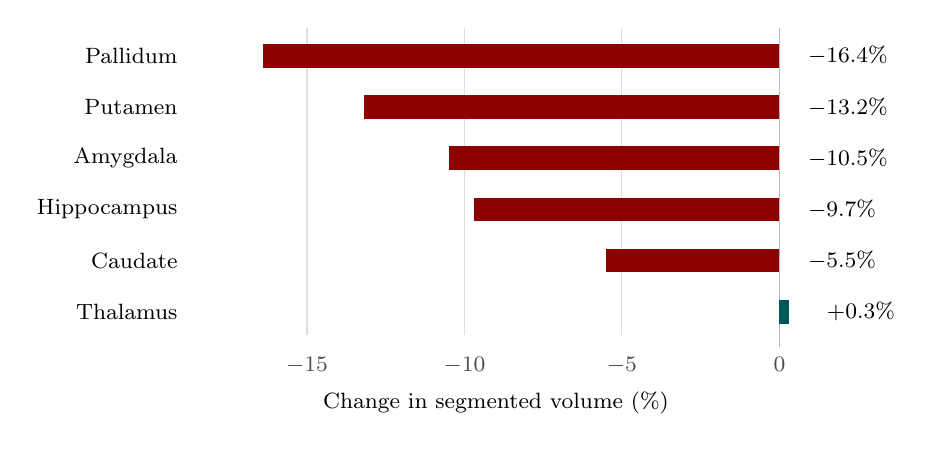
\begin{tikzpicture}[x=0.4cm, y=1cm]
    % --- gridlines and axis (1 unit of x = 1 percentage point) ---
    \foreach \t in {-15,-10,-5}{
      \draw[gray!25] (\t,0.35) -- (\t,-3.55);
      \node[font=\footnotesize, gray!60!black, anchor=north] at (\t,-3.70) {$\t$};
    }
    \draw[gray!55] (0,0.35) -- (0,-3.70);
    \node[font=\footnotesize, gray!60!black, anchor=north] at (0,-3.70) {$0$};
    \node[font=\footnotesize, anchor=north] at (-9,-4.15)
      {Change in segmented volume (\%)};

    % --- bars: (value, row y, label) ---
    \foreach \v/\y/\n in {%
      -16.4/0/Pallidum, -13.2/-0.65/Putamen, -10.5/-1.30/Amygdala,
      -9.7/-1.95/Hippocampus, -5.5/-2.60/Caudate}{
      \fill[red!55!black] (\v,\y-0.15) rectangle (0,\y+0.15);
      \node[font=\footnotesize, anchor=east] at (-18.8,\y) {\n};
      \node[font=\footnotesize, anchor=west] at (0.6,\y) {$\v\%$};
    }
    % thalamus is the one structure that gains volume
    \fill[teal!70!black] (0,-3.25-0.15) rectangle (0.3,-3.25+0.15);
    \node[font=\footnotesize, anchor=east] at (-18.8,-3.25) {Thalamus};
    \node[font=\footnotesize, anchor=west] at (1.2,-3.25) {$+0.3\%$};
  \end{tikzpicture}
  \caption{Volume change per structure. Bars grow leftward from zero because
    almost every structure shrinks. The thalamus, the structure with the most
    distinct borders, is the lone exception; the pallidum and putamen, which
    share a low-contrast boundary with each other, lose the most.}
  \label{fig:volume}
\end{figure}

% ---------------------------------------------------------------------
\section{Dice overlap}
% ---------------------------------------------------------------------

\begin{table}[htbp]
  \centering
  \caption{Dice coefficient between the structure segmented from the real volume
    and from the synthetic volume. The noise floor is the Dice obtained by
    re-segmenting the \emph{real} MR against the Phase~1 transported labels:
    identical anatomy, no synthesis. Headroom is the difference, i.e.\ the
    overlap still recoverable by improving synthesis.}
  \label{tab:dice}
  \begin{tabular}{l c r r}
    \toprule
    Structure & Dice & Noise floor & Headroom \\
    \midrule
    Thalamus    & \rpm{0.909}{0.022} & 0.977 & 0.068 \\
    Caudate     & \rpm{0.865}{0.046} & 0.971 & 0.105 \\
    Putamen     & \rpm{0.831}{0.046} & 0.967 & 0.136 \\
    Pallidum    & \rpm{0.731}{0.087} & 0.959 & 0.228 \\
    Hippocampus & \rpm{0.818}{0.046} & 0.966 & 0.148 \\
    Amygdala    & \rpm{0.835}{0.051} & 0.959 & 0.125 \\
    \midrule
    Mean        & 0.831              & 0.966 & 0.135 \\
    \bottomrule
  \end{tabular}
\end{table}

Dice is not saturated. The noise floor is tight (SD 0.007--0.015) relative to the
spread of the synthetic scores (SD 0.022--0.087), so the harness resolves a
change of about 0.01 Dice at $n=36$. The pallidum is the weakest structure by a
wide margin: $0.731\pm0.015$ against the thalamus at $0.909\pm0.004$, a gap of
roughly 12 standard errors.

% ---------------------------------------------------------------------
\section{Centroid displacement}
% ---------------------------------------------------------------------

\begin{table}[htbp]
  \centering
  \caption{Displacement of each structure's centre of mass between the real and
    the synthetic segmentation, in millimetres, computed with true voxel spacing.
    Image metrics are restricted to the structure: SSIM and CW-SSIM over its
    padded bounding box, PSNR masked to the structure itself.}
  \label{tab:centroid}
  \begin{tabular}{l c r r r}
    \toprule
    Structure & Centroid (mm) & SSIM & CW-SSIM & PSNR (dB) \\
    \midrule
    Thalamus    & \rpm{0.87}{0.34} & 0.680 & 0.658 & 26.12 \\
    Caudate     & \rpm{1.00}{0.63} & 0.728 & 0.689 & 24.01 \\
    Putamen     & \rpm{1.08}{0.47} & 0.646 & 0.652 & 26.21 \\
    Pallidum    & \rpm{1.50}{0.61} & 0.655 & 0.662 & 28.38 \\
    Hippocampus & \rpm{1.23}{0.67} & 0.583 & 0.608 & 20.95 \\
    Amygdala    & \rpm{0.98}{0.45} & 0.554 & 0.576 & 23.74 \\
    \midrule
    Mean        & 1.11             & 0.641 & 0.641 & 24.90 \\
    \bottomrule
  \end{tabular}
\end{table}

Every structure lies within approximately one voxel of ground truth.

% ---------------------------------------------------------------------
\section{Interpretation}
% ---------------------------------------------------------------------

CW-SSIM is constructed to be tolerant of small translations: a shift rotates the
phase of a complex wavelet coefficient while leaving its magnitude essentially
unchanged, and the index scores phase \emph{consistency} across a neighbourhood
rather than absolute phase. The implementation is verified translation-tolerant
(0.765 versus 0.636 for plain SSIM under a 2-pixel shift). Over the scored
structures, CW-SSIM and SSIM are nevertheless identical (0.641 versus 0.641,
Table~\ref{tab:centroid}): there is no misalignment for CW-SSIM to forgive. The
residual error is therefore intensity and texture \emph{within} the structure,
consistent with the sub-voxel centroid displacements.

This resolves an otherwise anomalous result. The pallidum has the worst Dice and
the worst centroid displacement, yet the \emph{highest} PSNR of any structure at
28.38\,dB. The pallidum is delimited by a low-contrast boundary against the
putamen rather than by a strong edge. Mild compression of that contrast moves
where the segmentation places the boundary, costing Dice and volume, while
leaving pixel-wise error small. The putamen, its neighbour across the same weak
border, is the second most affected structure; the thalamus, with the most
distinct borders, shows no volume deficit at all. The ordering of the volume
deficit by boundary contrast (Figure~\ref{fig:volume}) is the direct evidence for
this mechanism. Clinically this is the least convenient failure mode available,
as the globus pallidus internus is an established deep brain stimulation target.

% ---------------------------------------------------------------------
\section{Limitations}
% ---------------------------------------------------------------------

\paragraph{The measurements are of a segmenter, not of anatomy.}
Every figure compares SynthSeg applied to the real volume against SynthSeg
applied to the synthetic one. The noise floor bounds the segmenter's own
contribution at $0.966\pm0.01$ Dice, so approximately 3--4 points of the reported
deficit are attributable to the tool rather than to the model. It follows that
``the model under-fills the pallidum by 16\%'' and ``SynthSeg is conservative on
synthetic contrast'' are not separable from these measurements alone; the
defensible statement is that synthetic volumes \emph{segment} smaller.

\paragraph{The synthetic volumes are generated under a favourable protocol.}
The model is conditioned on a global intensity histogram of the target MR, and in
this evaluation that histogram is the ground-truth target's own. This is
defensible if framed as operator-supplied scanner calibration, but it is not a
deployment condition, and it inflates every figure downstream. A re-evaluation
conditioned on the training-set mean histogram, or on a template, yields the
deployment-realistic figure and should be reported alongside.

\paragraph{Exclusions.}
Ten of the 2160 structure-subject pairs in the full 180-subject cohort (0.46\%)
are excluded by the frozen Phase~1 quality-control manifest, where the reference
segmentation engulfs a lesion or abnormal tissue. No subject is dropped and the
test split remains $n=36$; all 432 pairs in this evaluation were scored
successfully.

\end{document}
